\documentclass[12pt]{book}
\usepackage{booktabs}
\usepackage[table]{xcolor}
\usepackage{tcolorbox}
\usepackage[T1]{fontenc}
\usepackage{wrapfig}
\usepackage{url}
\usepackage{dsfont}
\usepackage{enumitem}
\usepackage{array}
\usepackage{booktabs}

\usepackage{mathtools, nccmath}
\usepackage[polish]{babel}
\usepackage[utf8]{inputenc}
\usepackage{lmodern}
\usepackage{pifont}
\usepackage{blkarray, bigstrut}
\usepackage{amsmath}
\usepackage{kbordermatrix}
\usepackage{cases}
\usepackage{graphicx}
\usepackage{cellspace}
\usepackage[T1]{fontenc}
\usepackage{amsthm}
\selectlanguage{polish}
\usepackage{amsmath}
\usepackage{graphicx}
\usepackage{float}
\usepackage{cite}
\usepackage[margin=2.5cm]{geometry}
\theoremstyle{plain}
\newtheorem{definicja}{Definicja}
\newtheorem{twr}{Twierdzenie}
\newtheorem{lem}[twr]{Lemat}
\newtheorem{mur}{Murphy}[section]
\newcolumntype{P}[1]{>{\centering\arraybackslash}p{#1}}
\newcommand\green{\cellcolor{green!10}}
\newcommand\cincludegraphics[2][]{\raisebox{-0.5\height}{\includegraphics[#1]{#2}}}
\newcommand\red{\cellcolor{red!20}}
\newcommand\blue{\cellcolor{blue!20}}
\newcommand{\R}{\mathbb{R}}
\newcommand*{\tabbox}[2][t]{%
	\vspace{0pt}\parbox[#1][3.7\baselineskip]{1cm}{\strut#2\strut}}
\newcommand\addtag{\refstepcounter{equation}
	\renewcommand{\labelenumii}{\theenumii}
	\renewcommand{\theenumii}{\theenumi.\arabic{enumii}.}
	\tag{\theequation}}

\begin{document}
	\title{Optymalizacja  systemu sygnalizacji świetlnej w 
		oparciu o przepływowy model ruchu pojazdów.}
	\author{Michał Lis}
	\date{\today}
	\maketitle
	\tableofcontents
	
	\chapter {Środowiska symulacyjne i ich nauka}
	\section{Środowisko 4}
	\begin{figure}[H]
		\centering
		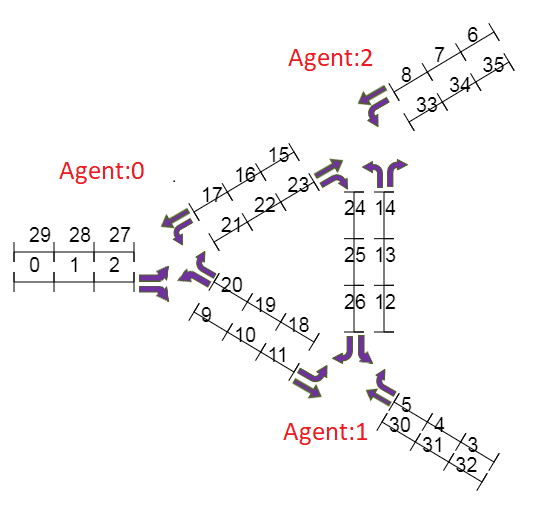
\includegraphics[width=10cm]{env_4_agenci}
		\label{fig:env_4_agenci}
		\caption{środowisko 4}
	\end{figure}
	
	Środowisko posiada 12 jednokierunkowych dróg. Każda droga ma 3 odcinki co daje w sumie 36 odcinków (są numerowane od 0 co widać na rysunku \ref{fig:env_4_agenci}).
	W sieci dróg znajdują się 3 skrzyżowania. Do każdego z nich jest przypisany agent, który odpowiada za sterowanie sygnalizacją świetlną.
	Pojazdy w jednym interwale czasowym pokonują jeden odcinek. Na skrzyżowaniach w przypadku zielonego światła przejeżdża maksymalnie 10 pojazdów w jedną stronę.
	
	
	\begin{figure}[H]
		\centering
		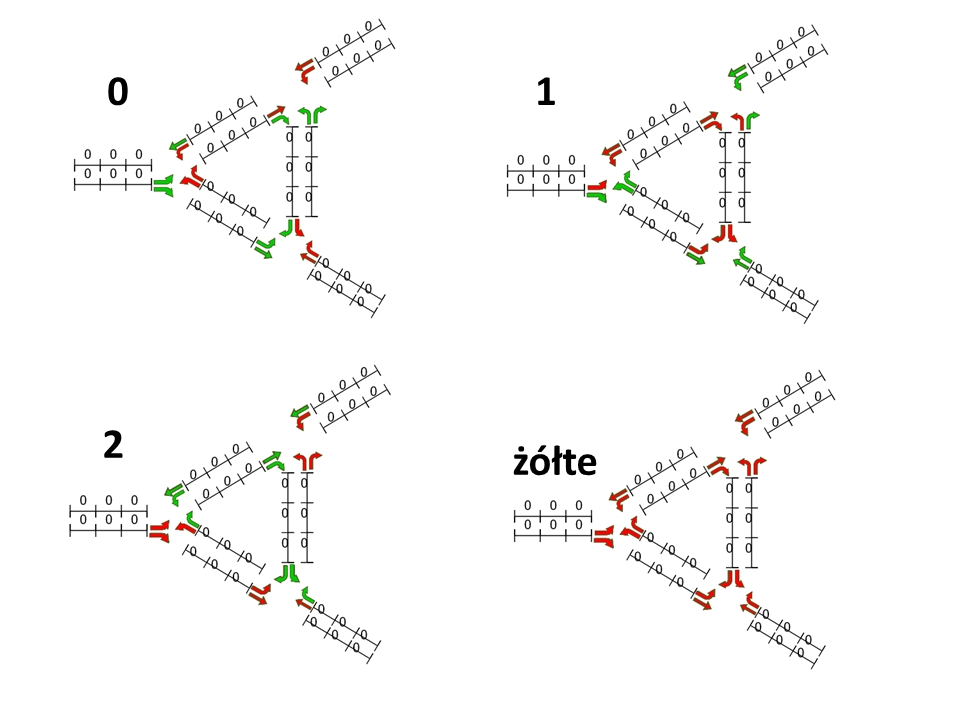
\includegraphics[width=14cm]{env_4_fazy}
		\label{fig:env_4_fazy}
		\caption{środowisko 4 - fazy świateł}
	\end{figure}
	Fazy świetlne: Każde skrzyżowanie posiada 4 fazy świetlne przedstawione powyżej. Fazy 0, 1 i 2 posiadają pewne zielone światła. Agent podejmuje decyzję o zmianie tych trzech faz. Zmiana faz świateł nie jest natychmiastowa i następuje dopiero po 2 interwałach czasowych fazy żółtych świateł. Agent może podjąć akcję a należącą do
	[0,1,2] w przypadku gdy obecna faza f należy do [0,1,2]. W pozostałym przypadku agent jest zobowiązany do przekazania akcji 'żółte'.
	
	\section{Uczenie Środowiska 4}	
	\subsection{Podejście 1}
	Każdy z trzech agentów jako stan przyjmuje 10 elementowy wektor. 9 elementów to ilości pojazdów na odcinkach będących przed skrzyżowaniem przypisanym do agenta. Wektor uzupełnia wartość obecnej fazy (0,1,2 lub 'żółte'). 
	Nagrody sa przyznawane jako suma pojazdów, które przejechały przez skrzyżowanie w trakcie najbliższych 4 interwałów czasowych. Początkowo przeprowadzana jest symulacja 100 epizodów z czego każdy trwa 90 interwałów czasowych. Ma ona na celu wygenerowania danych do treningu. Do nauki agent zapamiętuje jedynie te stany, których faza to 0, 1 lub 2. Nieistotne w procesie uczenia są stany z fazą 'żółte' gdyż agent ma tylko 1 możliwą decyzję do podjęcia. Do danych zapisywane są wartości stanu oraz nagród które zostały przydzielone dla pary stan-akcja. Następnie trenowana jest sieć neuronowa przyjmująca na wejście stan - 10 elementowy wektor. Sieć na wyjściu zwraca 3-elementowy wektor określający przewidziane nagrody dla akcji podjętej w zadanym stanie.
	Podsumowując dla wybranego agenta:
	\begin{itemize}
		\item \textbf{Stanem} są ilości pojazdów przed skrzyżowaniem oraz aktualna faza świetlna
		\item \textbf{Nagrodą} w chwili t jest suma pojazdów, które przejechały przez skrzyżowanie w trakcie najbliższych 4 interwałów czasowych czyli do momentu t+4.
		\item \textbf{Dane} są generowane poprzez przeprowadzenie 100 symulacji (każda ma 90 interwałów czasowych).
		\item \textbf{Sieć neuronowa} na podstawie wygenerowanych danych przewiduje najlepszą akcję dla obecnego stanu
		\item \textbf{Końcowa symulacja} zostaje przeprowadzona wedle przewidzianych przez sieć neuronową najlepszych akcji
	\end{itemize}
	
	
	Algorytm jest następujący:
	
	\begin{enumerate}
		\item 
		Utworzeni zostają 3 agenci dla poszczególnych skrzyżowań. Każdy z nich posiada sieć
		neuronową z 10 elementową warstwą wejściową i 3 elementową warstwą wyjściową.
		\item Przeprowadzone zostaje 50 losowych symulacji. Agenci zapamiętują dane z każdej chwili symulacji. Na te dane składa się stan oraz 3 elementowa tablica, która pod indeksem akcji przechowuje przydzieloną nagrodę. Pozostałe wartości tej 3 elementowej tablicy są przewidywane przez sieć neuronową. \label{item_100_episodes}
		\item Następuje trening sieci neuronowej. Parametry sieci neuronowej zostały wybrane w procesie walidacji krzyżowej. Zbiór walidacyjny to 0.2 wygenerowanego zbioru w punkcie \ref{item_100_episodes}. Pozostała część przeznaczona jest do treningu. Warunkiem stopu jest zwiększenie się błędu dla zbioru walidacyjnego.
		\item Agenci zapominają dane z przeprowadzonych 100 symulacji. Natomiast pozostawiają w pamięci wagi wytrenowanej siei neuronowej.
		\item Opcjonalnie w celu monitorowania postępów nauki przeprowadzona zostaje symulacja. Jej akcje są wybierane w sposób zachłanny. Dla aktualnego stanu zostaje zawsze wybrana akcja o najwyższej przewidzianej nagrodzie przez sieć.
		\item Powrót do kroku \ref{item_100_episodes}
	\end{enumerate}
	
	\subsection{Monitorowanie decyzji dla wybranego stanu}\label{subsec:env_4_monitorowanie_stanu}
\begin{figure}[h]
	\centering
	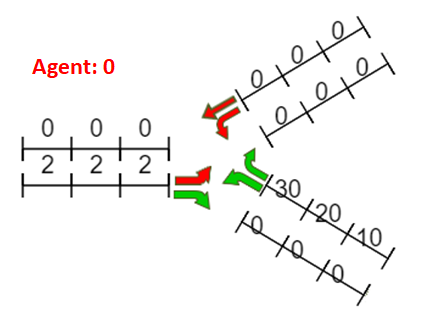
\includegraphics[width=12cm]{monitorowany_stan}
	\label{fig:monitorowany_stan}
	\caption{Monitorowany stan}
\end{figure}
W tej sekcji zostanie przedstawione jak zmieniały się rekomendowane przez agenta 0 akcje dla pewnego szczególnego stanu. Ilości pojazdów przed skrzyżowaniem to [2,2,2,30,20,10,0,0,0]. Aktualna faza świetlna to 1. Warto zadać sobie pytanie jaka akcja jest najbardziej opłacalna dla takiego stanu. Z pewnością warto podtrzymać aktualną fazę świetlną - gdyż przed tymi światłami jest najwięcej pojazdów. By osiągnąć ten cel należy wybrać akcję 1. Porządanym zjawiskiem jest, aby agent 0 dla tego stanu przewidywał największe nagrody dla akcji 1. Po każdej sesji uczenia sieci neuronowej zapisane zostały spodziewane nagrody. Ich wykres jest poniżej (każda pełna sesja algorytmu daje podobny wykres).
	\begin{figure}[H]
		\centering
		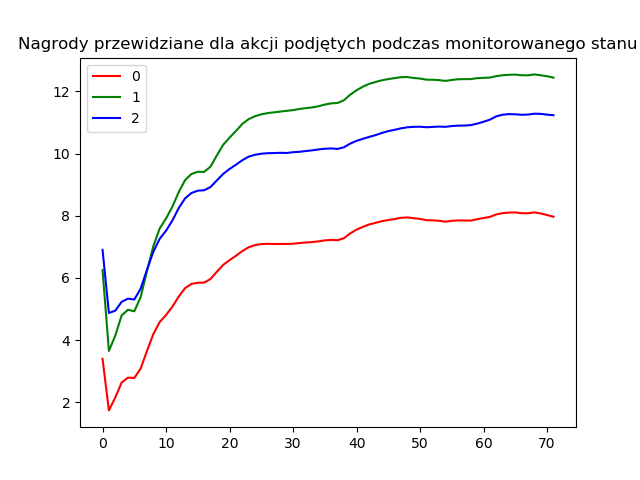
\includegraphics[width=14cm]{env_4_monitorowany_stan_wykres}
		\label{fig:env_4_monitorowany_stan_wykres}
	\end{figure}
	
	Zgodnie z przypuszczeniami z upływem czasu agent zauważa, że najlepszą akcją jest akcja 1. Jest to jak najbardziej dobry prognostyk. Niewiele gorszy wynik ma akcja 2 - zauważalnie lepszy od akcji 0. Ma to uzasadnienie w tym, że faza świetlna 2 ma zielone światło dla prawoskrętu przed najbardziej zatłoczoną drogą.


\section{Analiza wyników uczenia}	
	Wykres ilości pojazdów, które opuściły układ nie wygląda jakby wraz z upływem uczenia wynik się polepszał. Podobnie wygląda analogiczny wykres dla strategii losowych akcji. Należy zwrócić jednak uwagę iż średni wynik dla wyuczonej strategii to 1080. Do tego wyniku nie zbliżają się nawet najszczęśliwsze rezultaty dla losowych symulacji.
	
	\begin{figure}[H]
		\centering
		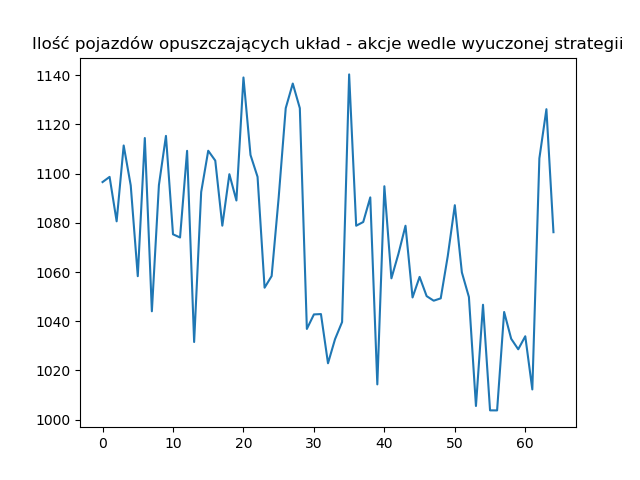
\includegraphics[width=13cm]{env_4_img_cars_out_policy}
		\label{fig:env_4_img_cars_out_policy}
	\end{figure}
		
	\begin{figure}[H]
		\centering
		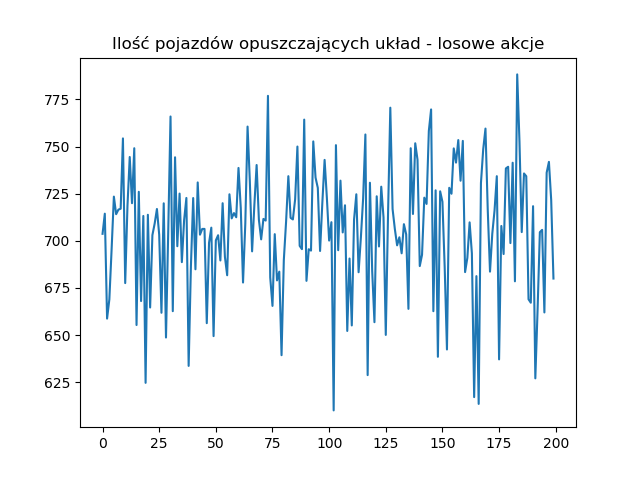
\includegraphics[width=14cm]{env_4_img_cars_out_random}
		\label{fig:env_4_img_cars_out_random}
	\end{figure}
\section{Monitorowanie kolejnego stanu}	
	Dla poprzednio monitorowanego stanu ukazanego w (\ref{subsec:env_4_monitorowanie_stanu}) sieć bardzo dobrze przewidywała najlepszą akcję. Był to jednak trywialny przykład z oczywistą do przewidzenia akcją. Należy prześledzić wyniki uczenia dla innego stanu. Z pewnością trudniej agentowi będzie podjąć poprawną decyzję dla następującego stanu. 
	\begin{figure}[H]
		\centering
		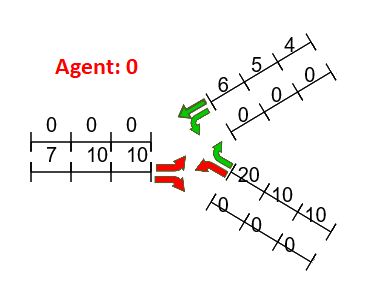
\includegraphics[width=10cm]{env_4_monitorowany_stan_2.png}
		\label{fig:env_4_monitorowany_stan_2.png}
	\end{figure}
	
	Przewidzenie najlepszej akcji (którą wydaje się być 2) nie sprawia agentowi większego kłopotu. Przeprowadzone zostało 5 pełnych sesji uczenia (każda po 10 minut) i wszystkie wyniki są bardzo podobne. Jedynie w jednej z nich były nieliczne momenty podczas których agent uznawał akcję 2 za najbardziej optymalną. Wykres przewidywanych nagród z tej sesji jest przedstawiony poniżej.  
	\begin{figure}[H]
		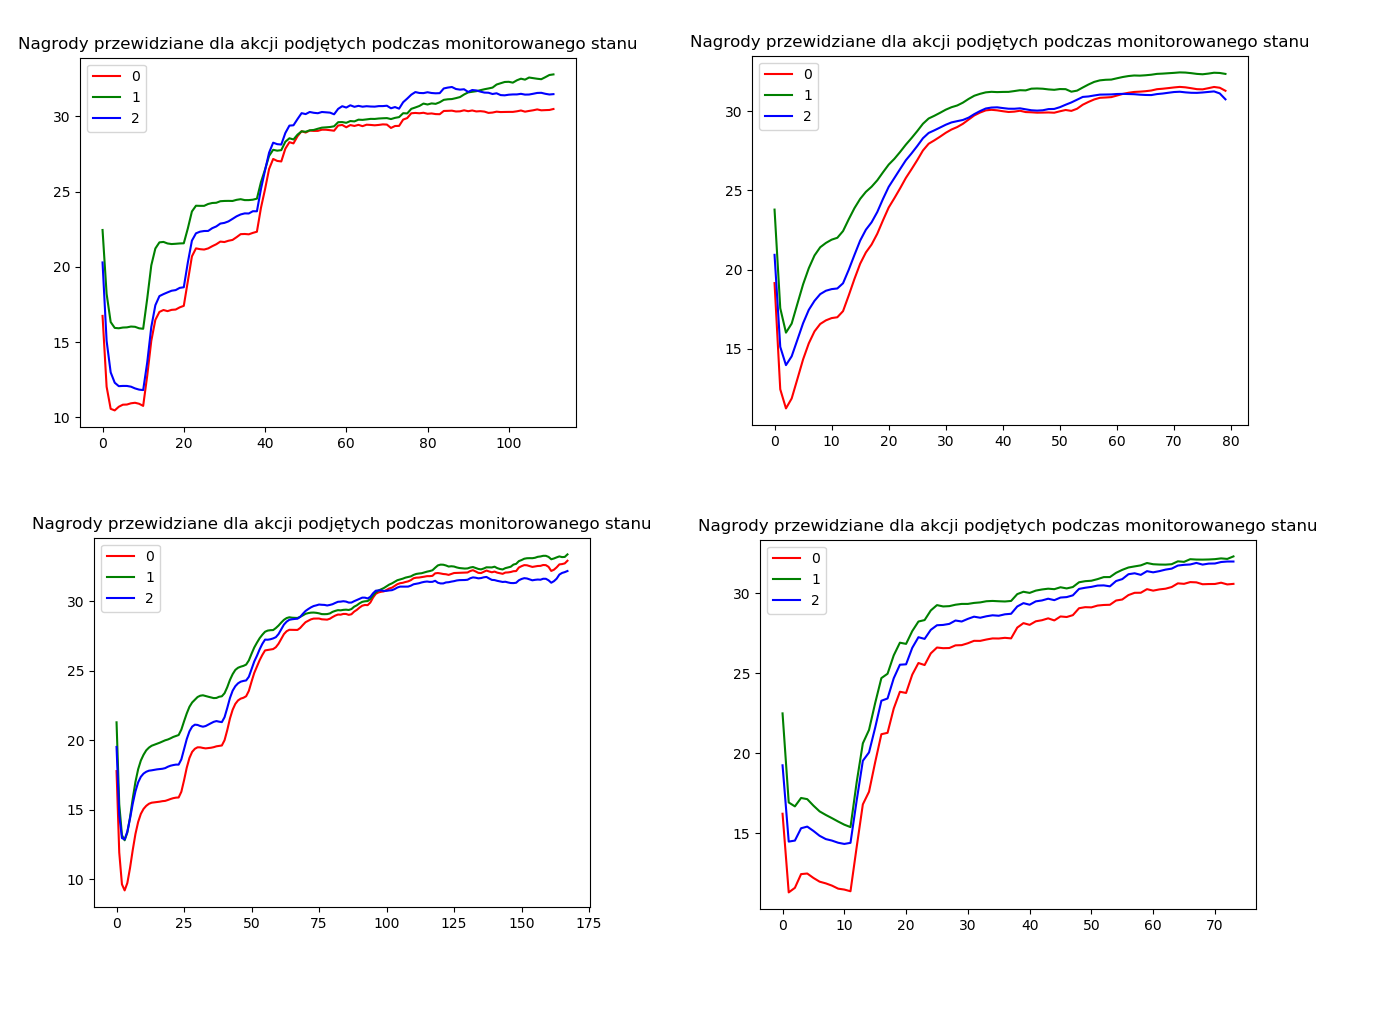
\includegraphics[width=20cm]{env_4_monitorowany_stan_2_ucz.png}
		\label{fig:env_4_monitorowany_stan_2_ucz.png}
	\end{figure}

Ten losowo wybrany stan, który wydaje się być wymagający w kwesti doboru najlepszej decyzji okazuje się nie sprawiać problemów dla agenta. Należy zatem prześledzić symulację, aby odnaleźć stany w których są podejmowane nieoptymalne akcje. Przykładowy stan z którym agent nie radzi sobie jest przedstawiony poniżej. 

\begin{figure}[H]
	\centering
	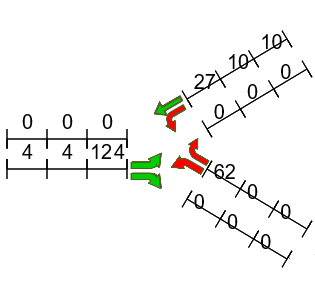
\includegraphics[width=10cm]{env4_3_monitorowany_stan.png}
	\label{fig:	env4_3_monitorowany_stan.png}
\end{figure}

Dobrym wyborem wydaje się być podtrzymanie fazy 0. Przez conajmniej 3 najbliższe interwały czasowe faza 0 gwarantuje przepływ 30 pojazdów w trakcie pojedynczego interwału. Warto zauważyć, że 30 przejeżdżających pojazdów przez skrzyżowanie to maksymalna ilość na 1 interwał. Pomimo tego argumentu agent zazwyczaj decyduje się na akcję 1. Chociaż faza 1 także wydaje się być dobra - to karencja w postaci żółtego światła na 2 interwały czasowe zdecydowanie przechyla szalę na korzyść akcji 0 i podtrzymania aktualnej fazy.



Wykonane zostaną następujące kroki, które potencjalnie mogą pozwolić agentowi uczyć się lepiej oraz odnajdywać poprawną akcję dla monitorowanego stanu.
- Epsilon-greedy learning - początkowo dane będą dalej generowane w pełni losowo. Z czasem uczenia do generowania danych używane będą także akcje dobrane wedle najwyższej oczekiwanej nagrody.
- Ciągła walidacja w trakcie uczenia
- Wprowadzenie możliwości ustanowienia stanu w środowisku i nauki dla niego.


\end{document} 













